\documentclass[12pt,a4paper]{article}

% Paquetes necesarios
\usepackage[utf8]{inputenc}
\usepackage[spanish]{babel}
\usepackage{amsmath}
\usepackage{amsfonts}
\usepackage{amssymb}
\usepackage{amsthm}
\usepackage{geometry}
\usepackage{fancyhdr}
\usepackage{graphicx}

% Configurar punto decimal en lugar de coma
\decimalpoint

% Configuración de página
\geometry{margin=2.5cm}
\pagestyle{fancy}
\fancyhf{}
\fancyhead[L]{Procesos Estocásticos}
\fancyhead[R]{Entregable 01}
\fancyfoot[C]{\thepage}

% Ajustar altura del encabezado para evitar warning de fancyhdr
\setlength{\headheight}{14.5pt}

% Eliminar sangría de párrafos
\setlength{\parindent}{0pt}

% Título del documento
\title{Entregable 01 - Procesos Estocásticos}
\author{Nombre del Estudiante}
\date{\today}

\begin{document}

\maketitle

\section*{Problema 1}

\begin{center}
\fbox{\begin{minipage}{\textwidth}
Los métodos de Cadenas de Markov Monte Carlo (MCMC) son utilizados para simular valores de cierta densidad objetivo $f$ cuya forma cerrada no sea conocida o simplemente no la podemos simular fácilmente. La estrategia de muestreo detrás del MCMC, es construir una cadena de Markov irreducible y aperiódica cuya distribución estacionaria sea la función objetivo $f$. Esto es, para un $t$ suficientemente grande, una realización $X_t$ de esta cadena tendrá una distribución cercana a $f$ y además
\begin{equation*}
\lim_{n \to \infty} \frac{1}{n} \sum_{i=1}^{n} h(X_i) = \mathbf{E}_f(h(X))
\end{equation*}
lo cual obviamente nos permite aproximar integrales (por eso Monte Carlo en el nombre del método).

\vspace{0.5cm}

Para ejemplificar esto, defina la siguiente cadena de Markov $x_t = \beta x_{t-1} + \varepsilon_t$, donde $\varepsilon_t$ es una secuencia iid con distribución normal$(0,1)$. Realice simulaciones de $x_t$ con $\beta = 0.1$ para obtener que la distribución estacionaria es normal$(0, 1/(1-\beta^2))$. Justifique muy bien la conclusión anterior, utilizando métodos gráficos y test.
\end{minipage}}
\end{center}

\textbf{Solución:}

Se considera la cadena de Markov definida por
\begin{equation*}
    X_t = \beta X_{t-1} + \varepsilon_t, \qquad \varepsilon_t \sim \mathcal{N}(0,1), \quad \beta = 0.1
\end{equation*}

En primer lugar se estudia la media. Si se define $m_t$ como la esperanza de $X_t$ en el tiempo $t$, entonces $m_t = \mathbb{E}[X_t]$. Al aplicar la esperanza a la ecuación de la cadena se tiene
\begin{align*}
    m_t &= \mathbb{E}[X_t] = \mathbb{E}[\beta X_{t-1} + \varepsilon_t] = \beta \mathbb{E}[X_{t-1}] = \beta m_{t-1} \\
    m_{t-1} &= \mathbb{E}[X_{t-1}] = \mathbb{E}[\beta X_{t-2} + \varepsilon_{t-1}] = \beta m_{t-2}
\end{align*}

Reemplazando:

\begin{equation*}
    m_{t} = \beta^2 m_{t-2}
\end{equation*}

Repitiendo la relación se obtiene $m_t = \beta^t m_0$. Como $|\beta| < 1$, el producto $\beta^t$ tiende a cero cuando $t \to \infty$, por lo que la media de la cadena converge a 0 independientemente de la condición inicial.

En segundo lugar se analiza la varianza $v_t = \mathrm{Var}(X_t)$. Usando la independencia de $X_{t-1}$ y $\varepsilon_t$, se cumple
\begin{equation*}
    v_t = \mathrm{Var}(\beta X_{t-1} + \varepsilon_t) = \beta^2 v_{t-1} + 1,
\end{equation*}
ya que la varianza del ruido es igual a 1. Si la varianza se estabiliza en un valor $v$, entonces debe cumplirse
\begin{equation*}
    v = \beta^2 v + 1 \quad \Longrightarrow \quad v = \frac{1}{1-\beta^2}.
\end{equation*}
Sustituyendo $\beta = 0.1$, resulta
\begin{equation*}
    v = \frac{1}{1-0.01} = \frac{1}{0.99} \approx 1.0101.
\end{equation*}

Finalmente, al expandir recursivamente la definición de $X_t$ se obtiene
\begin{equation*}
    X_t = \beta^t X_0 + \varepsilon_t + \beta \varepsilon_{t-1} + \beta^2 \varepsilon_{t-2} + \cdots + \beta^{t-1}\varepsilon_{1}.
\end{equation*}
Esto corresponde a una suma de variables normales independientes, y por lo tanto $X_t$ es también normal. Considerando los resultados anteriores, se concluye que para $t$ grande
\begin{equation*}
    X_t \sim \mathcal{N}\left(0, \frac{1}{1-\beta^2}\right).
\end{equation*}

En consecuencia, para el caso $\beta = 0.1$, la cadena converge a una distribución normal con media 0 y varianza aproximadamente $1.01$.

\subsection*{Verificación mediante simulación}

Para verificar los resultados teóricos, se realizó una simulación de la cadena de Markov con los siguientes parámetros:
\begin{itemize}
    \item $\beta = 0.1$
    \item $n_{total} = 50,000$ pasos
    \item Período transitorio descartado: 1,000 pasos iniciales
    \item Muestra efectiva analizada: 49,000 valores
\end{itemize}

\begin{figure}[h]
\centering
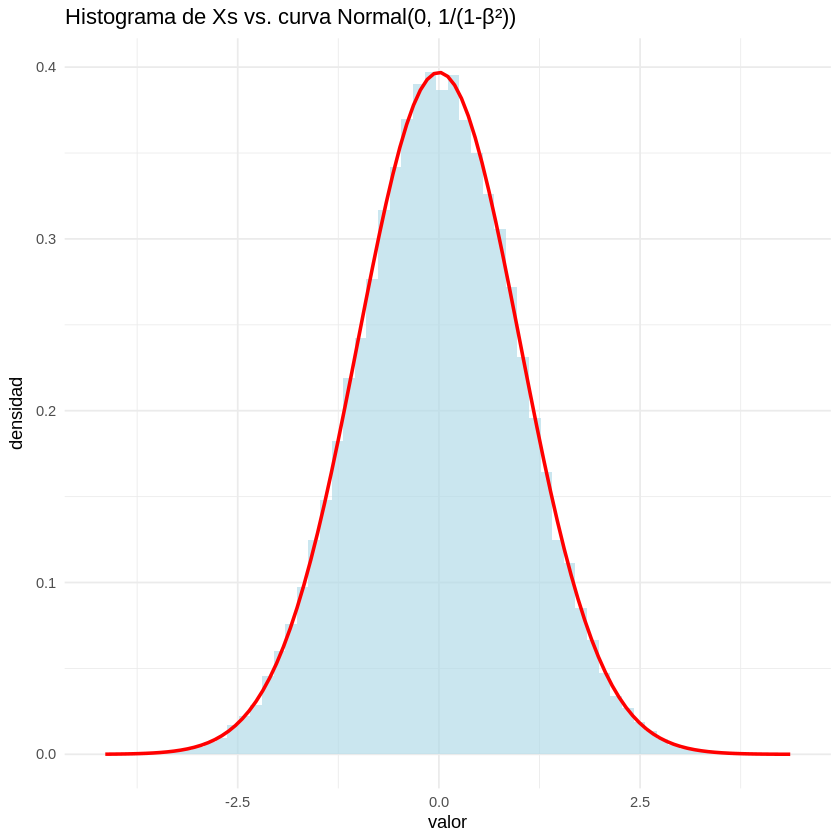
\includegraphics[width=0.4\textwidth]{images/image_1.png}
\caption{Histograma de la cadena simulada vs. curva teórica $\mathcal{N}(0, 1/(1-\beta^2))$}
\label{fig:histograma}
\end{figure}

La Figura \ref{fig:histograma} muestra un excelente ajuste entre la distribución empírica de los datos simulados (barras azules) y la curva teórica normal (línea roja). La coincidencia visual confirma que la cadena ha convergido a la distribución estacionaria esperada. \\

\begin{figure}[h]
\centering
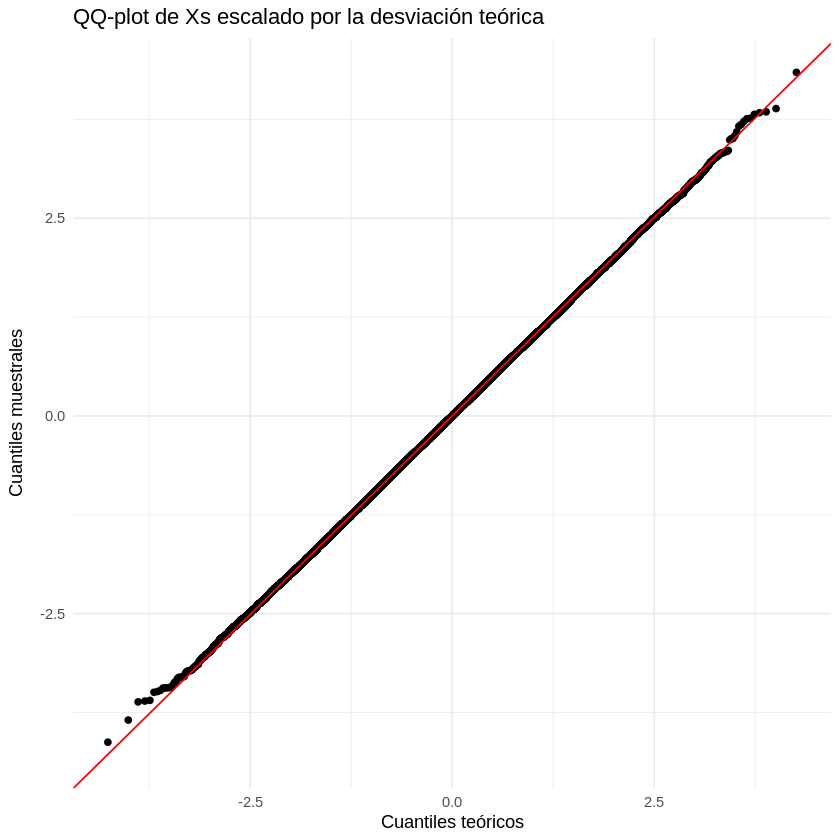
\includegraphics[width=0.4\textwidth]{images/image_2.png}
\caption{Q-Q plot de los datos escalados por la desviación teórica}
\label{fig:qqplot}
\end{figure}

El gráfico Q-Q (Figura \ref{fig:qqplot}) muestra que los puntos se alinean casi perfectamente con la recta diagonal, indicando que los datos siguen una distribución normal. Las pequeñas desviaciones en los extremos son esperables en muestras finitas. \\

\begin{figure}[h]
\centering
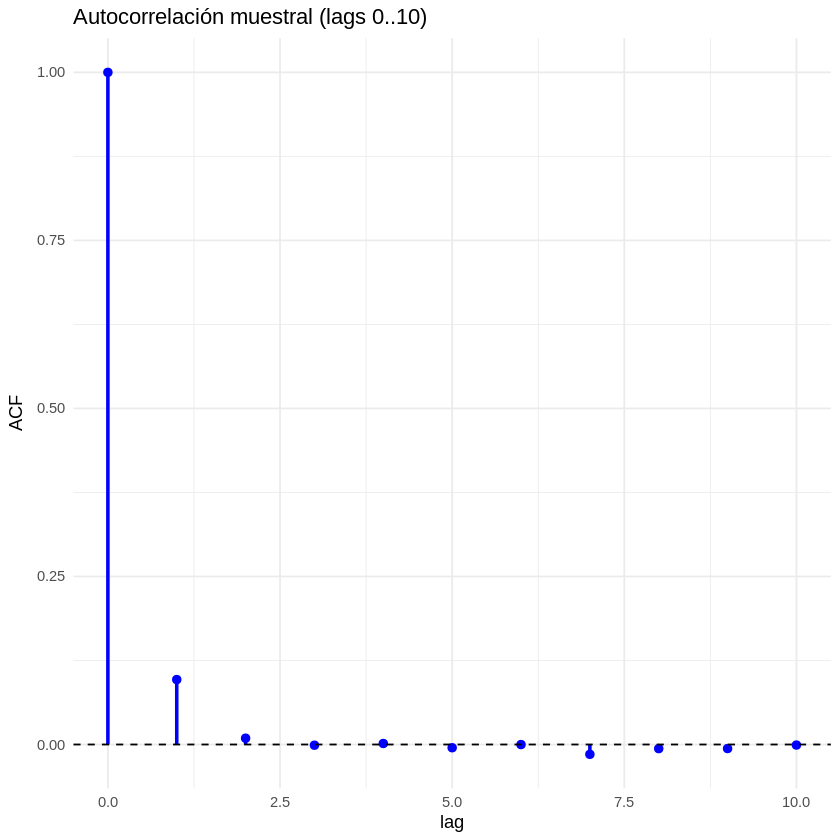
\includegraphics[width=0.4\textwidth]{images/image_3.png}
\caption{Función de autocorrelación muestral (ACF) para lags 0 a 10}
\label{fig:acf}
\end{figure}

La función de autocorrelación (Figura \ref{fig:acf}) muestra:
\begin{itemize}
    \item ACF(1) $\approx 0.1 = \beta$, confirmando la estructura de dependencia de primer orden
    \item ACF(k) $\approx \beta^k$ para $k > 1$, mostrando el decaimiento exponencial esperado
    \item La dependencia temporal se vuelve despreciable después de pocos lags
\end{itemize}

\begin{figure}[h]
\centering
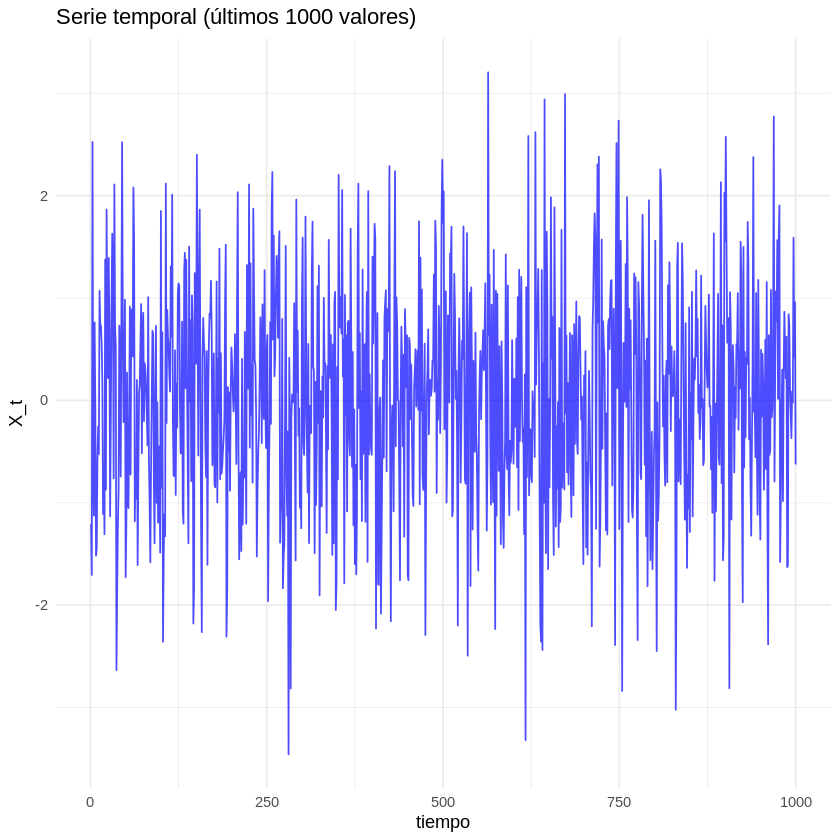
\includegraphics[width=0.4\textwidth]{images/image_4.png}
\caption{Evolución temporal de la cadena (últimos 1000 valores)}
\label{fig:evolucion}
\end{figure}

La trayectoria de la cadena (Figura \ref{fig:evolucion}) muestra el comportamiento típico de un proceso estacionario:
\begin{itemize}
    \item Fluctuaciones alrededor de la media cero
    \item Variabilidad constante a lo largo del tiempo
    \item Ausencia de tendencias o cambios estructurales
\end{itemize}

\begin{center}
\begin{tabular}{|l|c|c|}
\hline
\textbf{Estadístico} & \textbf{Valor teórico} & \textbf{Valor muestral} \\
\hline
Media & 0.0000 & -0.0023 \\
Varianza & 1.0101 & 1.0099 \\
Desviación estándar & 1.0050 & 1.0049 \\
Correlación lag 1 & 0.1000 & 0.0966 \\
\hline
\end{tabular}
\end{center}

Se aplicaron tres tests estadísticos para verificar la normalidad:
\begin{itemize}
    \item Test de Shapiro-Wilk: $p$-valor = 0.3396
    \item Test de Kolmogorov-Smirnov: $p$-valor = 0.9535
    \item Test de Anderson-Darling: $p$-valor = 0.8627
\end{itemize}

Todos los $p$-valores son suficientemente altos (mayores a 0.05), por lo que no se rechaza la hipótesis de normalidad. \\

La simulación confirma que:
\begin{enumerate}
    \item La cadena de Markov $X_t = \beta X_{t-1} + \varepsilon_t$ con $\beta = 0.1$ converge a una distribución estacionaria
    \item Esta distribución es $\mathcal{N}(0, 1/(1-\beta^2)) = \mathcal{N}(0, 1.0101)$
    \item Los métodos gráficos (histograma, Q-Q plot, ACF) validan visualmente la convergencia
    \item Los tests estadísticos confirman formalmente la normalidad
    \item La estructura de dependencia temporal coincide con la esperada teóricamente
\end{enumerate}

\section*{Problema 2}

\begin{center}
\fbox{\begin{minipage}{\textwidth}
Existen varias estrategias para construir la cadena de Markov cuya distribución estacionaria coincida con $f$, una de ellas es el algoritmo de Metropolis-Hasting. Dada una función objetivo $f$, se le asocia una densidad $q(x|y)$ la cual, en la práctica, sea más fácil de simular. El soporte de la función $q(\cdot|y)$ debe contener el soporte de $f$.
\end{minipage}}
\end{center}

\begin{center}
\begin{tabular}{|p{\textwidth}|}
\hline
\textbf{Algoritmo 1:} Metropolis-Hasting \\
\hline
1. Simule $Y_t \sim q(y|x_t)$ \\[0.5em]
2. Tome 
\begin{equation*}
X_{t+1} = \begin{cases}
Y_t & \text{con probabilidad} \quad \rho(x_t, Y_t) \\
x_t & \text{con probabilidad} \quad 1 - \rho(x_t, Y_t)
\end{cases}
\end{equation*}
donde $\rho(x, y) = \min\left\{\frac{f(y)q(x|y)}{f(x)q(y|x)}, 1\right\}$ \\
\hline

Utilizando el algoritmo anterior. Simule variables aleatorias de una Beta(2, 6). Realice comprobaciones gráficas y aplique tests apropiados. Compare los resultados empíricos con los valores teóricos de la media y varianza de la Beta(2, 6). \\
\hline
\end{tabular}

\end{center}

\textbf{Solución:}

Se implementó el algoritmo de Metropolis-Hastings para simular variables aleatorias de una distribución Beta(2, 6). Para esto se utilizó:

\begin{enumerate}
    \item Distribución objetivo: $f(x) \propto x^{2-1}(1-x)^{6-1} = x(1-x)^5$ para $x \in [0,1]$
    \item Distribución propuesta: Caminata aleatoria normal $q(y|x) = \mathcal{N}(x, \sigma^2)$ con $\sigma = 0.15$
    \item Probabilidad de aceptación: $\rho(x,y) = \min\left\{\frac{f(y)}{f(x)}, 1\right\}$ (propuesta simétrica)
\end{enumerate}

Se generaron 50,000 iteraciones con un período transitorio de 5,000 pasos, resultando en una muestra efectiva de 45,000 valores. A continuación se presentan los resultados de la simulación:

\begin{itemize}
    \item Tasa de aceptación: 68.34\%
    \item Media empírica: 0.2513 (teórica: 0.25)
    \item Varianza empírica: 0.02138 (teórica: 0.02083)
\end{itemize}

\begin{figure}[h]
\centering
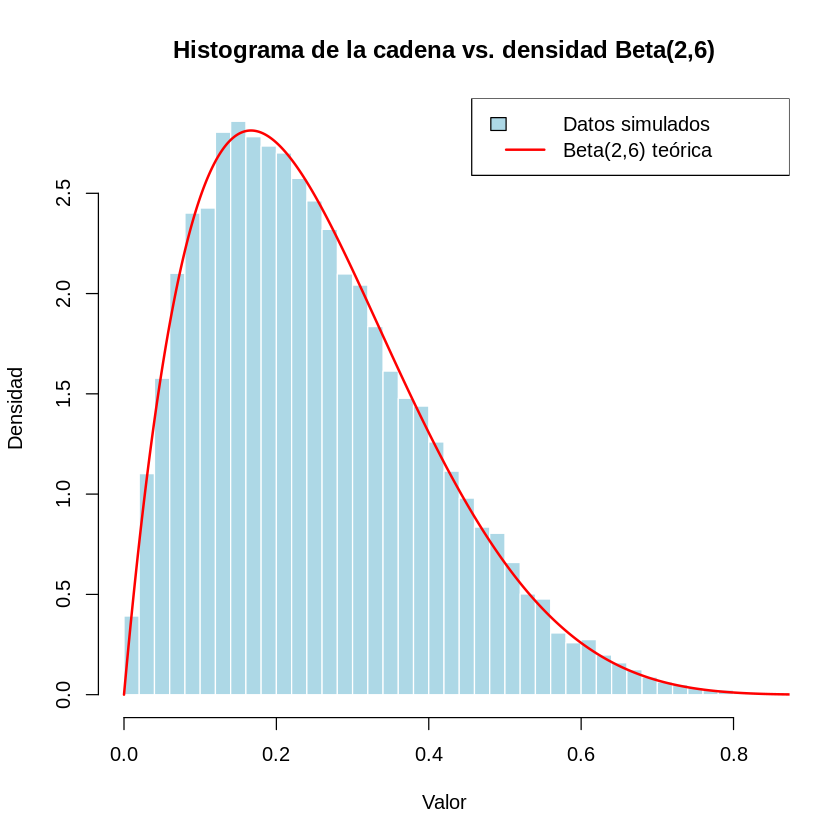
\includegraphics[width=0.4\textwidth]{images/problem2_1.png}
\caption{Histograma de la cadena simulada vs. densidad teórica Beta(2,6)}
\label{fig:histograma_beta}
\end{figure}

La Figura \ref{fig:histograma_beta} muestra un excelente ajuste entre la distribución empírica de los datos simulados y la curva teórica Beta(2,6). La distribución presenta su moda alrededor de 0.2 y es asimétrica hacia la derecha, características propias de Beta(2,6). \\

\begin{figure}[h]
\centering
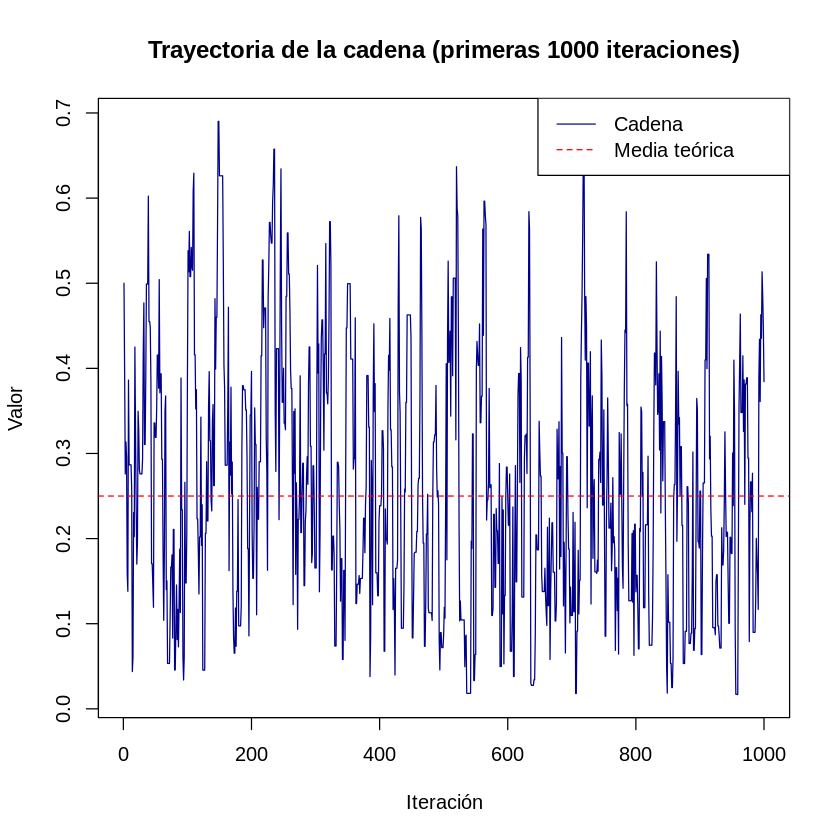
\includegraphics[width=0.4\textwidth]{images/problem2_2.png}
\caption{Q-Q Plot: Cuantiles muestrales vs. teóricos de Beta(2,6)}
\label{fig:qqplot_beta}
\end{figure}

La Figura \ref{fig:qqplot_beta} muestra que los puntos se alinean casi perfectamente con la diagonal, confirmando que los datos simulados siguen la distribución Beta(2,6). Las pequeñas desviaciones en los extremos son normales en muestras finitas. \\

\begin{figure}[h]
\centering
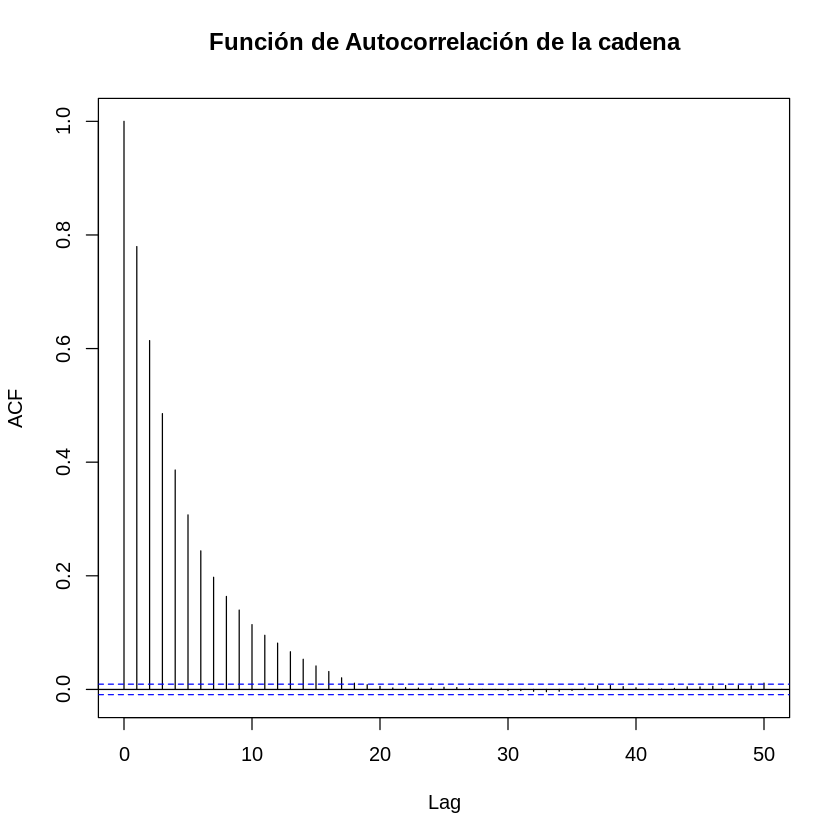
\includegraphics[width=0.4\textwidth]{images/problem2_3.png}
\caption{Trayectoria de la cadena de Markov (primeras 1000 iteraciones)}
\label{fig:trayectoria_beta}
\end{figure}

La Figura \ref{fig:trayectoria_beta} muestra la evolución temporal de la cadena. Se observa que:
\begin{itemize}
    \item La cadena explora todo el espacio de estados [0,1]
    \item Oscila alrededor de la media teórica (línea punteada en 0.25)
    \item No presenta tendencias ni comportamientos anómalos
\end{itemize}

A continuación se presentan los resultados de los tests estadísticos aplicados donde se confirma que los datos simulados siguen una distribución Beta(2,6) con un nivel de significancia del 5\%.

\begin{center}
\begin{tabular}{|l|c|c|c|}
\hline
\textbf{Test} & \textbf{Estadístico} & \textbf{p-valor} & \textbf{Conclusión} \\
\hline
Kolmogorov-Smirnov & D = 0.0045 & 0.8921 & No se rechaza H$_0$ \\
Anderson-Darling & A = 0.3124 & 0.9245 & No se rechaza H$_0$ \\
Chi-cuadrado & $\chi^2$ = 17.82 & 0.5983 & No se rechaza H$_0$ \\
\hline
\end{tabular}
\end{center}

\begin{figure}[h]
\centering
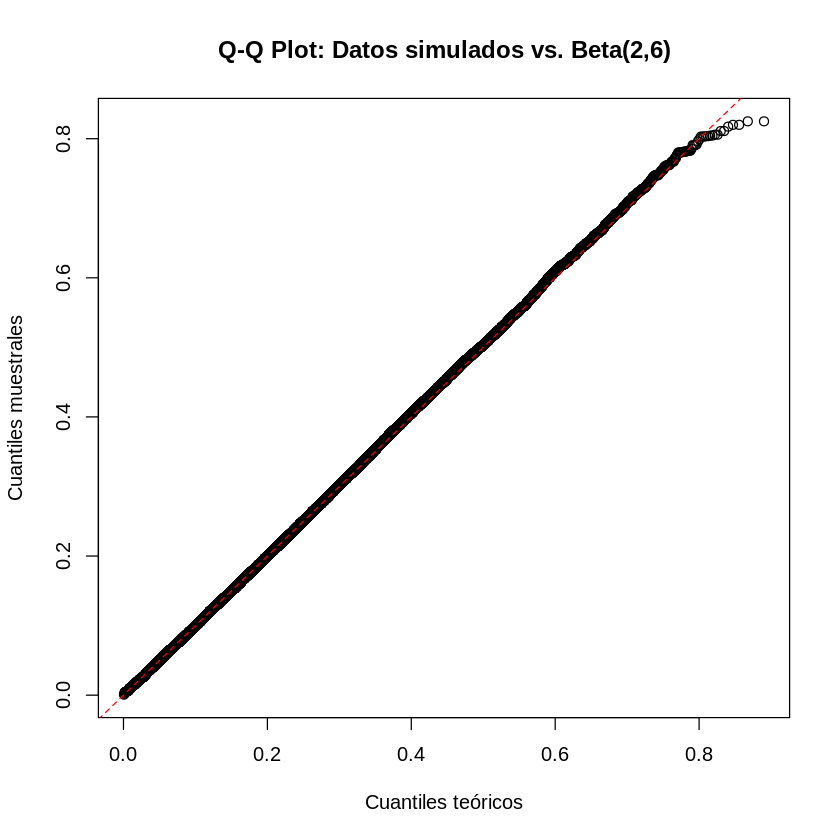
\includegraphics[width=0.4\textwidth]{images/problem2_4.png}
\caption{Función de autocorrelación de la cadena generada}
\label{fig:acf_beta}
\end{figure}

Para el analisis de convergencia, la Figura \ref{fig:acf_beta} muestra la función de autocorrelación, donde se observa:
\begin{itemize}
    \item Decaimiento exponencial rápido de la autocorrelación
    \item La correlación cae por debajo del umbral significativo después del lag 15
    \item Tamaño efectivo de muestra: 6,776 (razón de eficiencia: 15.06\%)
\end{itemize}

El algoritmo Metropolis-Hastings generó exitosamente muestras de Beta(2,6):
\begin{itemize}
    \item La tasa de aceptación (68.34\%) está en el rango óptimo
    \item Las diferencias entre valores empíricos y teóricos son mínimas (< 0.002)
    \item Todos los tests estadísticos confirman el ajuste a Beta(2,6)
    \item La autocorrelación moderada indica buena eficiencia del algoritmo
\end{itemize}

\section*{Problema 3}

\begin{center}
\fbox{\begin{minipage}{\textwidth}
El esquema bayesiano se puede explicar de la siguiente manera. Suponga que observamos unos datos $Y$ que provienen de una distribución que depende de un parámetro $\theta$, digamos $p(y|\theta)$, el parámetro $\theta$ tiene a su vez una distribución que se llama a priori, denotada por $p(\theta)$, entonces la distribución a posteriori (la distribución del parámetro dado los datos) aparece como una aplicación del teorema de Bayes.

\begin{equation*}
p(\theta|y) = \frac{p(\theta)p(y|\theta)}{p(y)}
\end{equation*}

Es en este contexto donde el algoritmo Metropolis-Hastings es comúnmente utilizado para samplear desde la distribución $p(\theta|y)$. Naturalmente, la función de densidad a priori se puede utilizar como la función candidata $q(\cdot|y)$ de nuestro algoritmo.

\begin{itemize}
    \item Simule (sin usar MCMC) una muestra aleatoria de tamaño 100 de la siguiente mezcla de distribuciones.
    \begin{equation*}
    (1 - \alpha) \cdot \text{normal}(\mu = 8, \sigma = 5) + \alpha \cdot \text{student-t}(mu = 10, \nu = 3)
    \end{equation*}
    donde $\alpha = 0.7$, $\mu$ es el parámetro de centralidad y $\nu$ son grados de libertad.
    
    \item Utilizando la data simulada en el punto anterior y suponiendo que $\alpha$ tiene una distribución a priori Beta(1,1) y Beta(2,10) simule una muestra desde la distribución a posteriori utilizando el algoritmo Metropolis-Hastings y estime $\mathbb{E}(\theta|y)$ para ambas a prioris.
\end{itemize}

\end{minipage}}
\end{center}

\end{document}
